\section{Execution Time Variation in Interactive Applications}
\label{sec:exec_time_prediction.applications}

%\subsection{Tasks and Jobs}
%
%% Tasks and jobs
%\begin{figure}
%  \begin{center}
%    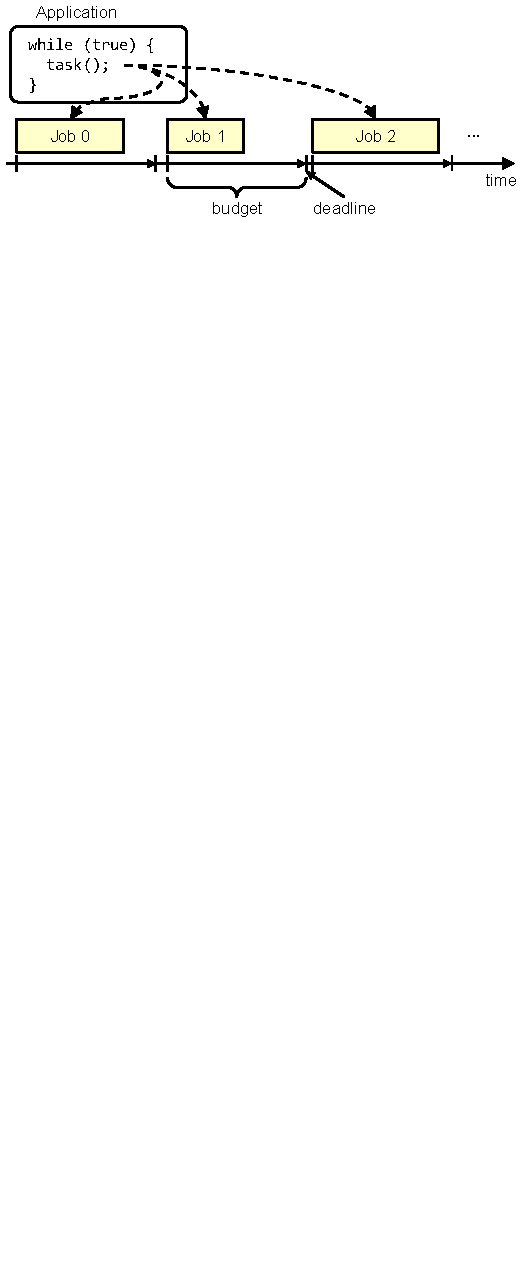
\includegraphics{exec_time_prediction/figs/jobs.pdf}
%    \caption{Example of tasks, jobs, and deadlines.}
%    \label{fig:exec_time_prediction.applications.jobs}
%  \end{center}
%\end{figure}
%
%We define a \emph{task} as a portion of an application that has an associated
%response-time requirement. We refer to the time period in which it must
%complete as its \emph{time budget}. For example, games are typically written
%with a main task that handles reading user input, updating game state, and
%displaying the output. In order to maintain a certain frame rate (e.g., 30
%frames per second), this task must finish within the frame period budget (e.g.,
%33 milliseconds for 30 frames per second operation).
%
%We define a \emph{job} as a dynamic instance of a task.
%Figure~\ref{fig:exec_time_prediction.applications.jobs} shows how a task maps
%to multiple jobs. Each job has a deadline which is the time by which it must
%finish execution. For example, for a game running at 30 frames-per-second, 30
%jobs for the game loop task are run each second. Each of these jobs has a
%deadline which is 33 milliseconds after the job's start time. These jobs all
%correspond to the same set of static task code, but their dynamic behavior
%differs due to different inputs and program state. For example, one job may see
%that the user has pressed a button and thus execute code to process this button
%press. Other jobs may see no new user input and skip the need to process user
%input.  As a result, job execution times can vary depending on input and
%program state.

\subsection{Variations in Execution Time}

% Execution time variation
\begin{figure}
  \begin{center}
    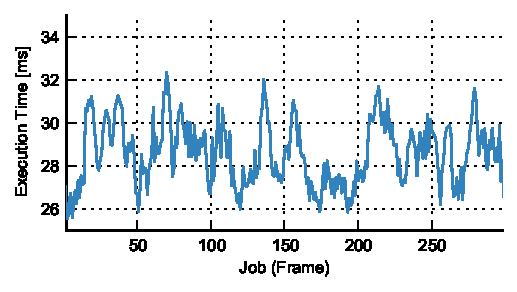
\includegraphics{exec_time_prediction/figs/ldecode_time.pdf}
    \caption{Execution time of jobs (frames) for ldecode (video decoder).}
    \label{fig:exec_time_prediction.applications.ldecode_time}
  \end{center}
\end{figure}

These variations in execution times between jobs can be significant.
Figure~\ref{fig:exec_time_prediction.applications.ldecode_time} shows the
execution time per job (frame) for a video decoder application (ldecode)
running on an ODROID-XU3 development board (see
Section~\ref{sec:exec_time_prediction.evaluation} for full experimental setup).
We can see that there are large variations in execution time from job to job
due to differences in input and program state when each job executes. Because
of this large variation, setting the appropriate DVFS level is a difficult
problem. 

Using a single DVFS level based on the average execution time (28.6
milliseconds) will lead to a number of jobs missing their deadline. On the
other hand, looking at the worst-case execution time (32.3 milliseconds)
implies that the application must be run at its maximum frequency, which means
that minimal energy saving from DVFS is possible. Instead, the large variations
from job to job imply that we need a fine-grained, per-job decision of the DVFS
level to use in order to minimize energy usage while avoiding deadline misses.

\subsection{Existing DVFS Controllers}
\label{sec:exec_time_prediction.applications.existing}

% Utilization
There are a large number of existing and proposed DVFS controllers. Most
controllers, such as the built-in Linux governors \cite{linux_governors},
adjust DVFS based on CPU utilization. When utilization is high, voltage and
frequency are increased, while when utilization is low, voltage and frequency
are decreased.  This does not explicitly take into account deadlines and can
result in high energy usage or deadline misses. For example, high CPU
utilization can cause a high voltage and frequency level to be used. However,
the time budget for the task may actually be very long and a lower voltage and
frequency would be sufficient, resulting in lower energy usage. Similarly, CPU
utilization for a job could be low due to memory stalls, causing the controller
to lower voltage and frequency levels. However, if the task has a tight time
budget, then this can result in a deadline miss, whereas running at higher
frequencies may have been able to meet the deadline.

% RT
DVFS has been explored in hard real-time systems in order to save energy while
guaranteeing that deadlines are met \cite{rtdvfs-systor12}. In order to ensure
that deadlines are never missed, the analysis must be strictly conservative
which limits the amount of energy that can be saved. That is, a task will
always be run at a frequency such that even the slowest jobs will meet the
deadline. 

% PID example
\begin{figure}
  \begin{center}
    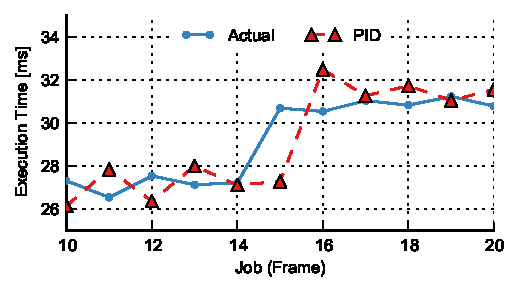
\includegraphics{exec_time_prediction/figs/ldecode_pid.pdf}
    \caption{Execution time of jobs (blue, solid) and execution time
    expected by a PID controller (red, dashed) for ldecode (video decoder).}
    \label{fig:exec_time_prediction.applications.ldecode_pid}
  \end{center}
\end{figure}

% Reactive
Other work has explored using run-time information to inform DVFS control in
the presence of deadlines. These approaches are largely reactive and use
information about past job execution times to predict future job times
\cite{gu-dac08, choi-iccad02, pegasus-isca14, nachiappan-hpca15}. This can
capture coarse-grained phase changes in execution time, but cannot capture the
fine-grained job-to-job variations in execution times as the adjustment in DVFS
level happens too late.  For example,
Figure~\ref{fig:exec_time_prediction.applications.ldecode_pid} shows the
expected execution times that a PID-based controller uses for setting the DVFS
level and the real execution times of the jobs. As we can see, the PID
controller's decision lags the actual execution times of the jobs.

% Specific
More recently, people have investigated predicting job execution time and
setting DVFS in order to meet deadlines for specific applications (e.g., game
rendering \cite{gu-rtas08}, web browsing \cite{zhu-hpca13, eqos-hpca15}, web
server/Memcached \cite{adrenaline-hpca15}). These approaches involved careful
analysis of the application of interest, requiring extensive programmer effort,
in order to design the controller. As a result, the resulting controllers
cannot be applied to other applications.

\subsection{Prediction-Based Control}

% Prediction-based control overview
\begin{figure}
  \begin{center}
    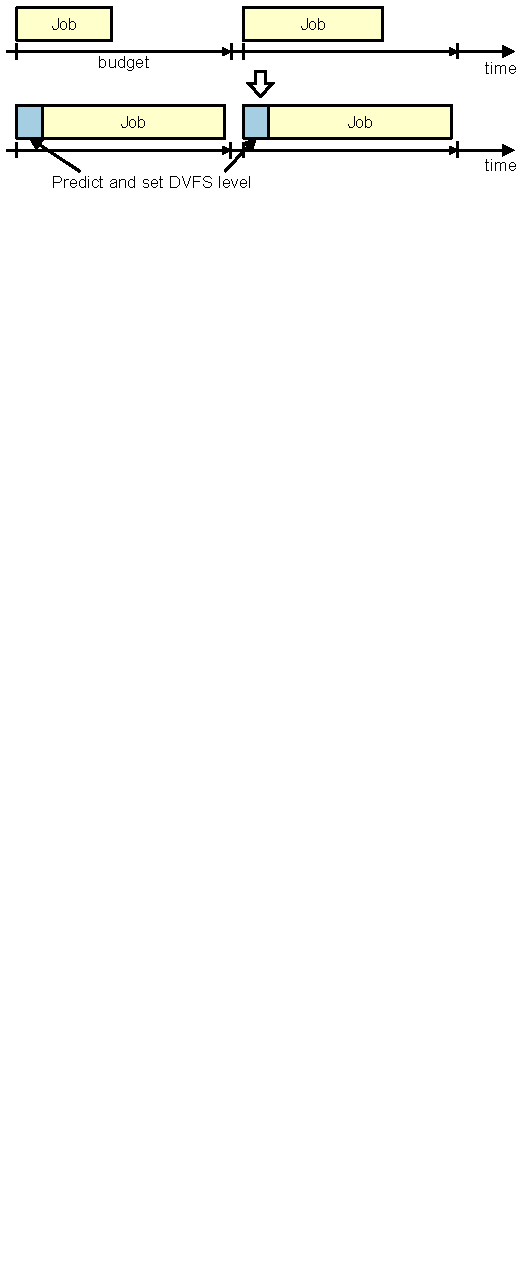
\includegraphics{exec_time_prediction/figs/prediction_overview.pdf}
    \caption{Overview of prediction-based control.}
    \label{fig:exec_time_prediction.applications.prediction_overview}
  \end{center}
\end{figure}

Our goal in this work is to develop a general and automated framework in order
to create prediction-based DVFS controllers that can minimize energy usage
without missing deadlines.
Figure~\ref{fig:exec_time_prediction.applications.prediction_overview} shows an
overview of the operation of our proposed prediction-based controller. The
basic idea is to pre-pend tasks with a small segment of code. This segment of
code will predict the appropriate DVFS level to use for each of the task's jobs
depending on the job's input and current program state.

The main source of execution time variation between jobs is due to different
inputs and program state. Thus, the main challenge in developing a
prediction-based DVFS controller is determining how to map job input and
program state values to the appropriate DVFS frequency level. In general,
finding a direct mapping from input values to frequency levels is challenging
because the mapping can be irregular and complicated. In addition, this mapping
varies from application to application. For example, for one application,
pressing the ``down'' key may correspond to a large increase in execution time
while for other applications it may have no effect on execution time. Our
solution is to take advantage of the program source to give us hints about how
input values and program state will affect execution time. We use the program
source to automatically generate a prediction-based DVFS controller.

